\documentclass[11pt]{article}

\RequirePackage{fontspec}

\usepackage{xcolor}

% Apple's text gray (from the cls)
\definecolor{fgcolor}{HTML}{333333}
\color{fgcolor}
\usepackage[margin=1in]{geometry}
\usepackage{amsmath,mathtools,amsthm}
\usepackage{unicode-math}

% TeX Gyre Pagella, a Palatino, with its matching math font. Loaded by filename
% because XeTeX resolves filenames through kpathsea and font names through
% fontconfig, and a TinyTeX install registers neither its serif nor its math
% faces with the latter. Loading by filename also means fontspec cannot guess
% the companion weights, so each is named.
\setmainfont{texgyrepagella-regular.otf}[
  BoldFont       = texgyrepagella-bold.otf,
  ItalicFont     = texgyrepagella-italic.otf,
  BoldItalicFont = texgyrepagella-bolditalic.otf,
]
\setsansfont{texgyreheros-regular.otf}[
  BoldFont   = texgyreheros-bold.otf,
  ItalicFont = texgyreheros-italic.otf,
  Scale      = MatchLowercase,
]
\setmonofont{texgyrecursor-regular.otf}[
  BoldFont = texgyrecursor-bold.otf,
  Scale    = MatchLowercase,
]
\setmathfont{texgyrepagella-math.otf}
% For a tighter page, swap the three faces above for LibertinusSerif-Regular.otf,
% LibertinusSans-Regular.otf and LibertinusMath-Regular.otf.
\usepackage{booktabs}
\usepackage{microtype}
\usepackage{enumitem}
\usepackage[authoryear,round]{natbib} % for \citet / \citep
\usepackage{graphicx}
\usepackage[colorlinks=true,allcolors=blue]{hyperref}

\newcommand{\E}{\mathbb{E}}
\newcommand{\Var}{\operatorname{Var}}
\newcommand{\Cov}{\operatorname{Cov}}
\newcommand{\tr}{\operatorname{tr}}
\newcommand{\ones}{\mathbf{1}}
\newcommand{\HT}{\mathrm{HT}}
\newcommand{\pos}[1]{\left(#1\right)_+}


% Every computed number on the page comes from here, and this file is written by
% benchmarks/make_exhibits.py. Nothing measured is typed into the prose.
% Generated by benchmarks/make_exhibits.py. Do not edit.
\newcommand{\PanelUsers}{1,134}
\newcommand{\PanelDomains}{64,074}
\newcommand{\PanelVisits}{6,236,834}
\newcommand{\LabeledDomains}{34,078}
\newcommand{\LabelCoverage}{53.2}
\newcommand{\LabeledVisitShare}{76.4}
\newcommand{\EvalUsers}{1,132}
\newcommand{\EvalDensity}{0.27}
\newcommand{\TruthNorm}{11.1}
\newcommand{\NumClasses}{2}
\newcommand{\NumCoefficients}{26}
\newcommand{\BetaRows}{13}
\newcommand{\BetaCols}{2}
\newcommand{\EffAtTwoFifty}{0.113}
\newcommand{\EffFactorAtTwoFifty}{9}
\newcommand{\EffRatioLo}{0.062}
\newcommand{\EffRatioHi}{0.113}
\newcommand{\RmseAtTwoThousand}{1.18}
\newcommand{\RelErrAtTwoThousand}{11}
\newcommand{\SrsCoverageLo}{0.84}
\newcommand{\SrsCoverageHi}{0.88}
\newcommand{\PpsCoverageLo}{0.938}
\newcommand{\PpsCoverageHi}{0.952}
\newcommand{\SrsSkew}{8.5}
\newcommand{\PpsSkew}{0.5}
\newcommand{\SrsVarDispersion}{5.3}
\newcommand{\PpsVarDispersion}{0.5}
\newcommand{\SrsVarRatio}{1.01}
\newcommand{\PpsVarRatio}{0.99}
\newcommand{\CubeSeExcess}{10}
\newcommand{\CubeReps}{500}
\newcommand{\CubeCoverage}{0.96}
\newcommand{\NormMedian}{9}
\newcommand{\NormMax}{72,260}
\newcommand{\OracleFactor}{2.8}
\newcommand{\ShrinkGainSmall}{46}
\newcommand{\ShrinkGainMid}{20}
\newcommand{\ShrinkGainLarge}{5}
\newcommand{\ZeroFillBiasLo}{14}
\newcommand{\ZeroFillBiasHi}{53}
\newcommand{\Reps}{300}
\newcommand{\FrontierReps}{200}
\newcommand{\HeadlineBudget}{250}
\newcommand{\BudgetShareAtTwoThousand}{6}
\newcommand{\ReproMaxDiff}{0.004}
\newcommand{\ReproTolerance}{0.02}


\title{Estimand-Driven Sampling of Reusable Labels}
\author{Gaurav Sood}
\date{}

\begin{document}
\maketitle

\begin{abstract}
Labeling \LabeledDomains{} websites is a month of work; labeling 250 of them is an afternoon. On a metered browsing panel we show that the afternoon buys almost the same regression coefficients, provided the 250 are chosen by how much each site moves the estimate and weighted by the chance it had of being chosen. Sampling websites with probability proportional to influence attains \EffAtTwoFifty{} of the error that spending the same budget uniformly at random incurs, holds that ratio across a twentyfold range of budgets, and produces intervals that cover at their nominal rate where uniform sampling's cover at \SrsCoverageLo{}. The argument rests on an identity rather than an approximation: writing $V$ for row shares and $H=(X^\top X)^{-1}X^\top V$, the complete-label coefficient is $\beta^*=\sum_j h_j a_j$, so an item's entire contribution to the answer is fixed before any label is bought. From that identity we derive the optimal inclusion probabilities, show that the certainty head of a take-all design falls out of a constraint rather than a judgment call, give the take-some boundary in closed form, and show that the criterion has to be declared because fitted-value and coefficient loss can disagree on a fifth of a budget. We also show where the guarantee stops. When the purchased label builds a covariate rather than an outcome, an unbiased input yields an attenuated coefficient, and we give the correction the design makes available. The methods are implemented in an open-source package, and every number below regenerates from a hashed extract distributed with it.
\end{abstract}

\section{Introduction}

Some labels are expensive and get reused. A website's content category, a merchant's industry, a surname's likely ethnicity: each costs something to determine once, and then applies to every record touching that entity. A browsing panel of a thousand people generates millions of visits across tens of thousands of domains, and an analyst who wants to know whether older adults encounter more trackers must attach a label to the domains, not to the visits. The labeling bill scales with the number of distinct entities; the value of a label scales with how much of the data it touches and with what the analyst intends to estimate. Those two quantities are not the same, and the gap between them is the opportunity.

The usual response is to label as much as the budget allows, most valuable first, and treat what remains as zero. That is a reasonable instinct and it produces a biased estimate whose bias cannot be bounded from the data, because the unlabeled entities contribute an amount that depends on labels nobody bought. The alternative this paper develops is to treat the labeling decision as a sampling problem: give every entity that matters a positive and known chance of selection, choose those chances to minimize the variance of the estimate you actually want, and weight by the reciprocal.

That reframing is not new in outline. Business surveys have long taken all the large units and sampled the rest; case-cohort designs measure expensive covariates on every case plus a random subcohort \citep{Prentice1986}; high-influence probability sampling picks units by their anticipated contribution to a regression \citep{Clark2022}. What is specific here is that the purchased label attaches to an entity reused across many records through a map the analyst already knows, and that this makes the value of a label exact rather than anticipated. Writing $V$ for the matrix of row shares and $H=(X^\top X)^{-1}X^\top V$ with columns $h_1,\dots,h_m$, the complete-label regression coefficient decomposes with no remainder:
\[
\beta^*=\sum_{j=1}^m h_j a_j .
\]
Item $j$ contributes $h_j a_j$ and nothing else, and $h_j$ is computable from the usage counts and the covariates before a single label is purchased. Every result below is a consequence of that identity.

We contribute four things. First, the design: the risk-minimizing inclusion probabilities are $\pi_j^\star=\min\{1,\lambda\sqrt{b_j/c_j}\}$, in which the cap at one produces a certainty head rather than presuming one, and the take-all boundary of the simpler uniform-tail design has a closed form that replaces a judgment call with an arithmetic one. Second, the estimand must be declared: fitted-value loss and coefficient loss weight items differently and can disagree on a fifth of a budget, and there is a diagnostic for the populations on which the choice provably cannot matter. Third, the limits of the guarantee: when the label builds a covariate rather than an outcome, an unbiased constructed variable produces an attenuated coefficient, which we correct using the fact that the design knows its own error variance; and the reported standard error separates into a component the budget controls and one it cannot, whose ratio tells an analyst when to stop paying. Fourth, an open-source implementation \citep{fewlab}, in which the three objects this argument keeps distinct---a ranking, a probability design, and a realized sample---are distinct types, so that the mistake of weighting a deterministic selection as though it were a sample cannot be expressed.

We evaluate on a population where the answer is known. A metered browsing panel of \PanelUsers{} US adults was scanned for tracking behavior, and \LabeledDomains{} of its \PanelDomains{} domains returned a successful scan. Restricting to those domains makes the complete-label coefficient exactly computable, so every design is scored against the same fixed target instead of against an estimate of one.

\section{Setup and an exact decomposition}

Let $C=(c_{ij})\in\mathbb{R}_+^{n\times m}$ be counts of unit $i$'s activity on item $j$, let $T_i=\sum_j c_{ij}$, and let $V_{ij}=c_{ij}/T_i$ be row shares. Item $j$ carries a latent label $a_j$, and the unit-level outcome is the share of activity on labeled items,
\[
y_i=\sum_{j=1}^m V_{ij}\,a_j .
\]
With covariates $X\in\mathbb{R}^{n\times p}$ the estimand is the complete-label regression coefficient $\beta^*=(X^\top X)^{-1}X^\top y$. Units with $T_i=0$ have no shares and are excluded.

Collecting $H=(X^\top X)^{-1}X^\top V$ with columns $h_j$ gives
\begin{equation}
\label{eq:decomposition}
\beta^*=(X^\top X)^{-1}X^\top V a=\sum_{j=1}^m h_j a_j .
\end{equation}
This is an identity. There is no error term, no distributional assumption, and no approximation of a covariance: item $j$'s entire contribution to the estimand is $h_j a_j$, and $h_j$ depends only on $(C,X)$. The algebra carries a vector label $a_j\in\mathbb{R}^q$ unchanged, with $\beta^*=\sum_j h_j a_j^\top$, so a mutually exclusive taxonomy and a coder's probability distribution over classes need no separate treatment.

Sample items with inclusion probabilities $\pi_j\in(0,1]$ and indicators $I_j$ that do not depend on the unknown labels. The Horvitz--Thompson estimator \citep{HorvitzThompson1952}
\begin{equation}
\label{eq:ht}
\widehat\beta=\sum_{j=1}^m \frac{I_j}{\pi_j}h_j a_j
\end{equation}
is design-unbiased for $\beta^*$, since $\E[I_j/\pi_j]=1$ and everything else in \eqref{eq:decomposition} is fixed. Unbiasedness is thus a constraint on the design, not a property to be hoped for: it holds exactly when every item with $h_j\neq 0$ receives positive probability and enters with weight $1/\pi_j$.

Two consequences deserve emphasis because they are what deterministic selection gives up. An item that no unit touched has $h_j=0$, contributes nothing, and may be left unlabeled at no cost in bias; this is the only case in which $\pi_j=0$ is correct. And selecting the top $K$ items by any criterion assigns probability one above the cut and zero below it, so its bias is $-\sum_{j\notin S}h_ja_j$, a quantity that depends on labels nobody purchased and therefore cannot be estimated or bounded from the data in hand.

\section{What an item is worth}

Under independent item sampling the estimator's error is $\widehat\beta-\beta^*=\sum_j(I_j/\pi_j-1)h_ja_j$, so for a positive semidefinite $W$ the loss $\tr[W(\widehat\beta-\beta^*)(\widehat\beta-\beta^*)^\top]$ has exact design risk
\begin{equation}
\label{eq:risk}
\E_p\,L=\sum_{j=1}^m \frac{1-\pi_j}{\pi_j}\,b_j,\qquad b_j=(h_j^\top W h_j)\,a_j^2 .
\end{equation}
The criterion enters only through $b_j$, and it has to be chosen. Fitted-value loss sets $W=X^\top X$ and gives $g_j^\top(X^\top X)^{-1}g_j$ for $g_j=X^\top v_j$. Coefficient loss sets $W=I$ and gives $h_j^\top h_j=g_j^\top(X^\top X)^{-2}g_j$. A contrast $L^\top\beta^*$ sets $W=LL^\top$ and gives $\|L^\top h_j\|^2$. All three yield square-root allocations and convex programs. On a well-conditioned $X^\top X$ they rank items almost identically; they diverge when $X^\top X$ is far from a scaled identity and the $h_j$ span several directions, where in our experiments they disagreed on roughly a fifth of a top-$K$ set. There is no target-free notion of which items are worth labeling, and reporting one criterion while computing another is a mistake we have made ourselves.

\paragraph{Labels that need no pilot.} For a mutually exclusive taxonomy $a_j^\top a_j=1$, so $b_j=h_j^\top W h_j$ is known before any labeling begins and the optimal design can be computed from usage data alone. When labels are counts rather than class indicators the squared norms vary and a pilot sample or a proxy is required; \S\ref{sec:evidence} measures what that knowledge is worth.

\paragraph{When the criterion cannot matter.} If every $h_j$ points in the same direction and items differ only in magnitude, then $b_j\propto\|h_j\|^2$ under every $W$, all criteria induce the same ordering, and the choice of estimand is immaterial. Expected counts of the form $\text{activity}_i\times\text{popularity}_j$ produce exactly this degeneracy, and a simulation built on such a population will report every design as equivalent whatever it measures. The singular values of the column-normalized $H$ diagnose it, read against a noise floor of order $1/\sqrt{\bar c}$ for average count $\bar c$, since integer counts inject spurious directions at that scale.

\section{Designs}

\paragraph{Clipped probability proportional to size.} Minimizing \eqref{eq:risk} subject to $\sum_j c_j\pi_j=K$ and $\pi_j\le 1$ gives
\begin{equation}
\label{eq:pps}
\pi_j^\star=\min\!\left\{1,\ \lambda\sqrt{b_j/c_j}\right\}
\end{equation}
for the $\lambda$ that exhausts the budget. The cap is not a separate rule for large items: the set on which it binds \emph{is} the certainty head, and in a heavy-tailed population it absorbs most of the budget. The square-root rule also settles the unbiasedness constraint without further intervention, since it assigns strictly positive probability to every item with $b_j>0$. A probability floor is therefore unnecessary for unbiasedness, and imposing one moves the design away from minimum risk; its only legitimate purpose is to bound the largest weight.

\paragraph{A certainty core with a uniform tail.} Order the contributions $b_1\ge\cdots\ge b_m$, take the first $H$ with certainty, and give the remainder the common probability $p_H=(K-H)/(m-H)$. With $S_H=\sum_{j>H}b_j$ the risk is
\begin{equation}
\label{eq:core}
R(H)=\frac{m-K}{K-H}\,S_H ,
\end{equation}
so the boundary follows from evaluating at most $K$ cutoffs, and promoting one more item into the core pays exactly when $b_{H+1}>S_H/(K-H)$. Two qualifications. Equation \eqref{eq:core} is exact for a Bernoulli tail; drawn as a fixed-size simple random sample the variance is smaller, because fixing the count removes the sample-size variability and contributions enter centered. Read it as a planning criterion and an upper bound. And the design cannot beat \eqref{eq:pps}, which varies the tail probabilities. Its appeal is operational: a uniform tail is a simple random sample, easy to specify to a vendor, easy to audit, and equipped with a variance estimator any reader can check.

\paragraph{Turning probabilities into a list.} A design is not a draw. Include every item with $\pi_j^\star=1$, then draw the remainder to exact size with first-order inclusions $\pi^\star$ and balancing auxiliaries $g_j$, using the cube method \citep{DevilleTille2004}. Balancing drives $\sum_j(I_j/\pi_j-1)g_j$ toward zero, which shrinks the realized error for any labels whatsoever, and costs nothing in unbiasedness because the first-order probabilities are unchanged. Estimation then uses the probabilities the sampler \emph{delivered}. If a sampler rescales the requested probabilities, as a fixed-size sampler must, the delivered vector is the one that makes \eqref{eq:ht} unbiased.

\paragraph{The reverse problem.} Fixing a per-unit precision instead of a budget, and minimizing the number of labels subject to $\sum_j q_{ij}/\pi_j\le\varepsilon_i^2+\sum_j q_{ij}$ for $q_{ij}=V_{ij}^2$, is convex with the same square-root shape $\pi_j^\star\propto\sqrt{\sum_i\mu_iq_{ij}/c_j}$. It is always feasible, since $\pi\equiv 1$ makes the design variance vanish.

\section{Using a cheap classifier}

Suppose a frozen classifier supplies a prediction $\mu_j$ for every item at negligible cost. The difference estimator
\begin{equation}
\label{eq:diff}
\widehat\beta_\mu=\sum_{j=1}^m h_j\mu_j+\sum_{j=1}^m\frac{I_j}{\pi_j}h_j(a_j-\mu_j)
\end{equation}
is design-unbiased whatever the classifier says, because the first term is a known constant and the second corrects it without bias. A poor classifier costs variance and never bias, so there is no risk in supplying one. The risk becomes $\sum_j\frac{1-\pi_j}{\pi_j}(h_j^\top Wh_j)\,\E(a_j-\mu_j)^2$, so acquisition should target influence times residual label uncertainty: for a calibrated binary probability $p_j$ that residual is $p_j(1-p_j)$, and for calibrated one-hot probabilities it is $1-\|\mu_j\|^2$, both known without labels. Plugging predictions directly into a regression instead is what produces the bias and overconfidence documented by \citet{FongTyler2021}; here the correction is made by the design rather than by a model of the prediction error.

\section{When the label builds a covariate}
\label{sec:covariate}

Everything above puts the purchased label in the outcome. Reverse it, and the central guarantee fails. Suppose the target is $\gamma$ in
\[
z_i=\gamma\,y_i+x_i^\top\delta+\epsilon_i
\]
where $y$ must again be constructed from labels. Substituting an unbiased $\widehat y=y+u$ regresses on a covariate measured with error, so $\gamma$ is \emph{attenuated} and not merely noisy. Unbiasedness of $\widehat y$ offers no protection, and the attenuation does not shrink with the size of the panel: it shrinks only with the labeling budget. On a synthetic population with $\gamma=2$ we measure a naive estimate of about $1.4$.

What makes the problem tractable is that the measurement error was created deliberately. The design chose $\pi$, so $\Var(u)=\sum_j\frac{1-\pi_j}{\pi_j}a_j^2v_jv_j^\top$ is known up to the labels, and the sample estimates it without bias. Residualizing on the controls with $M_X$, the naive slope $\widetilde y^\top\widetilde z/\widetilde y^\top\widetilde y$ has a denominator inflated by $\E[u^\top M_Xu]$, and subtracting the estimate
\[
\widehat{\Delta}=\sum_{j\in S}\frac{1-\pi_j}{\pi_j^2}\,a_j^2\,\bigl(v_j^\top M_X v_j\bigr)
\]
removes the first-order attenuation. The correction is a ratio with a reduced denominator, so it overshoots: in the same experiment it moves an estimate that was $30$ percent low to one about $10$ percent high. That is a large improvement and not an exact fix, and intervals should come from redrawing the design rather than from a closed form.

The design target changes too, and in an instructive direction. The outcome case rewards items whose exposure is \emph{aligned} with $X$, through $h_j^\top W h_j$. A covariate's coefficient is identified by the variation in $\widetilde y$ that survives residualizing, so the relevant quantity is $v_j^\top M_X v_j=\|v_j\|^2-h_j^\top X^\top X h_j$, the exposure \emph{orthogonal} to $X$. In principle these are complementary. In practice they are not far apart, because with many more units than covariates the orthogonal part dominates the squared norm; in our experiments the two scores correlate above $0.99$ and the better-targeted design improves root mean squared error by under ten percent. The lesson is the reverse of the outcome case: here the choice of design matters little and the failure to correct for attenuation matters a great deal.

\section{Inference}
\label{sec:inference}

\paragraph{Two variances, and only one is for sale.} Writing $\sigma^2$ for the residual variance of $y$ on $X$,
\[
\Var(\widehat\beta)=\underbrace{\sigma^2(X^\top X)^{-1}}_{\text{$n$ units}}+\underbrace{\textstyle\sum_j\frac{1-\pi_j}{\pi_j}b_j}_{\text{$K$ labels}} .
\]
Only the second term falls as the budget grows, so the ratio is a stopping rule: once the design term sits well below the first, further labels buy almost nothing and the binding constraint is the size of the panel. Estimating $\sigma^2$ requires care, because the residuals of $\widehat y$ on $X$ carry design noise as well as regression error. That noise contributes $\sum_j\frac{1-\pi_j}{\pi_j}a_j^2(\|v_j\|^2-h_j^\top X^\top Xh_j)$ to the residual sum of squares; subtracting it leaves an unbiased estimator rather than an inflated one.

\paragraph{Fixed-size draws are covered conservatively.} The Poisson expression \eqref{eq:risk} is exact for independent Bernoulli trials. Fixing the sample size and balancing on auxiliaries both remove variation it still counts, so a cube draw's true variance is smaller than the figure reported. Measured on the panel of \S\ref{sec:evidence}, the reported standard error exceeds the realized spread by \CubeSeRatioLo{} to \CubeSeRatioHi{} percent and coverage runs to \CubeCoverage{} against a nominal $0.95$. Sen--Yates--Grundy estimators with joint inclusion probabilities would tighten this \citep{Sen1953,YatesGrundy1953}; we report the conservative bound.

\paragraph{Buying bias on purpose.} Shrinking the weight so item $j$ enters with $\alpha_j/\pi_j$ is weight trimming \citep{Potter1990,Beaumont2013}. It is defensible here because the price is computable in advance: the bias is bounded by $\sum_j(1-\alpha_j)\|h_j\|\,|a_j|$, which for a mutually exclusive taxonomy needs no labels, and which the classifier of \eqref{eq:diff} converts from a bound into an estimate. Setting $\alpha_j=\pi_j$, so every labeled item enters with weight one and unlabeled items are treated as zeros, is the common practice of zero-filling; it is a point on this frontier and \S\ref{sec:evidence} finds it is never the best one.

\section{Evidence}
\label{sec:evidence}

We evaluate on a population whose labels are entirely known, so that every design is scored against the same fixed target rather than against an estimate of one. The panel is YouGov Pulse: \PanelUsers{} US adults metered for June 2022, \PanelVisits{} visits across \PanelDomains{} registered domains \citep{PulseData}. Each domain was submitted to Blacklight for a seven-measure tracking audit, and \LabeledDomains{} scans succeeded, covering \LabelCoverage{} percent of domains and \LabeledVisitShare{} percent of visits \citep{BlacklightData}. The evaluation frame is those domains, and it is \EvalDensity{} percent dense.

The outcome is the published per-user exposure rate, which is exactly $y=Va$, and the regression is the published specification of exposure on gender, race, education, and age group. Fitting it on all \LabeledDomains{} labels reproduces the published coefficients to within $0.004$ against a stated replication tolerance of $0.02$, which establishes that the exercise targets the same quantity the substantive paper does. With \NumClasses{} label measures reduced to the two headline ones, $\beta^*$ is $\BetaRows\times\BetaCols$ and $\|\beta^*\|=\TruthNorm$. Each row of Table~\ref{tab:evidence} is \Reps{} independent Poisson draws from the same finite population, so the reported spread is design variance alone.

\begin{table}[t]
\centering\small
% Generated by benchmarks/make_exhibits.py. Do not edit.
\begin{tabular}{rlrrrrr}
\toprule
$K$ & Design & RMSE & RMSE/SRS & Bias & Coverage & Core \\
\midrule
250 & Uniform & 52.9 & 1.000 & 2.6 & 0.869 & 0 \\
250 & Core + uniform tail & 25.6 & 0.483 & 1.2 & 0.912 & 105 \\
250 & Clipped PPS & 5.97 & 0.113 & 0.24 & 0.942 & 26 \\
250 & Clipped PPS, $a_j^2$ known & 2.13 & 0.040 & 0.14 & 0.949 & 38 \\
\midrule
1,000 & Uniform & 26.4 & 1.000 & 1.5 & 0.872 & 0 \\
1,000 & Core + uniform tail & 7.02 & 0.266 & 0.47 & 0.937 & 552 \\
1,000 & Clipped PPS & 2.29 & 0.087 & 0.13 & 0.945 & 185 \\
1,000 & Clipped PPS, $a_j^2$ known & 0.604 & 0.023 & 0.028 & 0.950 & 311 \\
\midrule
2,000 & Uniform & 19.1 & 1.000 & 0.79 & 0.877 & 0 \\
2,000 & Core + uniform tail & 3.1 & 0.163 & 0.15 & 0.943 & 1,176 \\
2,000 & Clipped PPS & 1.18 & 0.062 & 0.047 & 0.952 & 550 \\
2,000 & Clipped PPS, $a_j^2$ known & 0.268 & 0.014 & 0.017 & 0.947 & 791 \\
\bottomrule
\end{tabular}

\caption{Labeling designs scored against the complete-label coefficient matrix $\beta^*$, whose own Frobenius norm is \TruthNorm{}. RMSE and bias are Frobenius norms of the error in $\widehat\beta$, in the units of $\beta^*$. Coverage is the share of nominal 95 percent intervals containing the truth, pooled over \NumCoefficients{} coefficients. Core is the number of items the cap in \eqref{eq:pps} places at probability one, which the design produces rather than the analyst choosing. Population: \EvalUsers{} panelists and \LabeledDomains{} domains with known tracking labels; \Reps{} Poisson draws per row. Budgets of 100 and 500 are omitted for space and interpolate.}
\label{tab:evidence}
\end{table}

\begin{figure}[t]
\centering
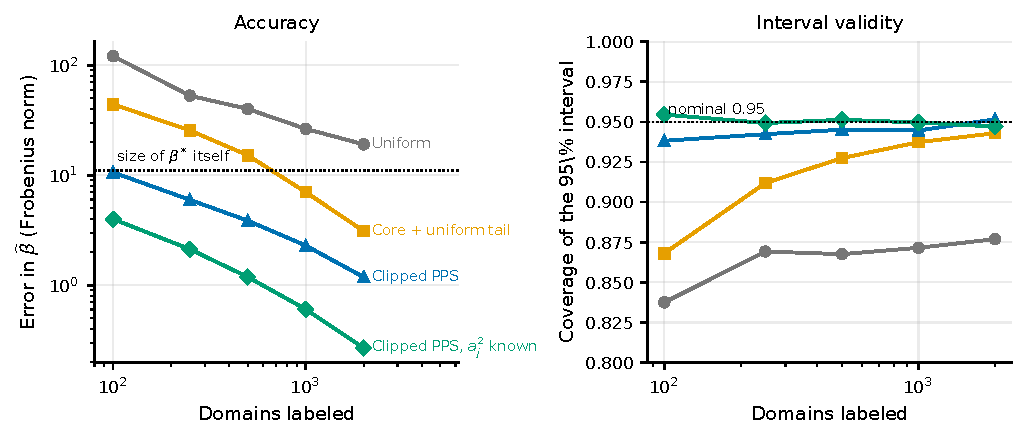
\includegraphics{generated/fig_efficiency.pdf}
\caption{Accuracy and interval validity against the labeling budget, for the four designs of Table~\ref{tab:evidence}. Left: Frobenius norm of the error in $\widehat\beta$, with a reference line at the norm of $\beta^*$ itself, so a series near the line is no better than reporting zero. Right: coverage of the nominal 95 percent interval, reference line at $0.95$. Both axes are logarithmic in the budget. Population and replication as in Table~\ref{tab:evidence}.}
\label{fig:efficiency}
\end{figure}

Four features of Table~\ref{tab:evidence} and Figure~\ref{fig:efficiency} carry the argument.

Every design is unbiased, including the poor one. Uniform sampling's bias at $K=250$ sits within a Monte Carlo standard error of zero. The designs differ in variance and not in bias, which is what a probability design guarantees and what separates this exercise from zero-filling, whose bias is real and unbounded.

The efficiency ratio is flat in the budget. Clipped PPS holds between \EffRatioLo{} and \EffRatioHi{} of the uniform error across a twentyfold range of $K$, so the gain is a property of the design rather than of a fortunate operating point. At $K=2{,}000$ its error is \RmseAtTwoThousand{}, or \RelErrAtTwoThousand{} percent of the size of the quantity being estimated, from labeling six percent of what was actually labeled.

Intervals from a good design cover and intervals from a poor one do not. Uniform sampling covers at \SrsCoverageLo{} to \SrsCoverageHi{} against a nominal $0.95$, and the cause is not a faulty variance estimator: over repeated draws it recovers the true variance to a ratio of \SrsVarRatio{}. What fails is the normal approximation. Under uniform sampling a few very high influence domains either enter the sample or do not, leaving $\widehat\beta$ skewed at \SrsSkew{} with a variance estimate whose own standard deviation is \SrsVarDispersion{} times its mean; under PPS those figures are \PpsSkew{} and \PpsVarDispersion{}. The design that shrinks the interval is also what makes the interval mean anything, and reporting a standard error from a badly allocated sample is the more dangerous of the two failures because it looks like an answer.

Knowing the squared label norms is worth a further factor of \OracleFactor{}. Blacklight labels are counts rather than class indicators, with squared norms running from a median of \NormMedian{} to a maximum of \NormMax{}, so the simplification $a_j^\top a_j=1$ does not apply. That gap measures what a pilot sample or the classifier of \eqref{eq:diff} is worth on this population, and it is the largest single improvement available.

\begin{table}[t]
\centering\small
% Generated by benchmarks/make_exhibits.py. Do not edit.
\begin{tabular}{rrrrr}
\toprule
$K$ & $\alpha$ & Bias & SD & RMSE \\
\midrule
250 & 0.00 & 5.86 & 1.01 & 5.95 \\
250 & 0.25 & 4.38 & 2.01 & 4.82 \\
250 & 0.50 & 2.91 & 3.29 & \textbf{4.39} \\
250 & 0.75 & 1.44 & 4.62 & 4.84 \\
250 & 0.90 & 0.579 & 5.43 & 5.46 \\
250 & 1.00 & 0.245 & 5.97 & 5.97 \\
\midrule
1,000 & 0.00 & 3.72 & 0.599 & 3.76 \\
1,000 & 0.25 & 2.79 & 0.943 & 2.95 \\
1,000 & 0.50 & 1.87 & 1.38 & 2.32 \\
1,000 & 0.75 & 0.947 & 1.83 & \textbf{2.06} \\
1,000 & 0.90 & 0.409 & 2.12 & 2.16 \\
1,000 & 1.00 & 0.159 & 2.31 & 2.31 \\
\midrule
4,000 & 0.00 & 1.53 & 0.188 & 1.55 \\
4,000 & 0.25 & 1.15 & 0.26 & 1.18 \\
4,000 & 0.50 & 0.772 & 0.349 & 0.848 \\
4,000 & 0.75 & 0.392 & 0.446 & 0.594 \\
4,000 & 0.90 & 0.165 & 0.506 & \textbf{0.532} \\
4,000 & 1.00 & 0.0331 & 0.546 & 0.547 \\
\bottomrule
\end{tabular}

\caption{Bias and variance as the Horvitz--Thompson weight is shrunk. The same items are labeled in every row and only the weight differs: at $\alpha=1$ it is $1/\pi_j$ and the estimator is unbiased, and at $\alpha=0$ every labeled item enters with weight one, which is what zero-filling the unlabeled amounts to. Bold marks the smallest RMSE in each block. Population as in Table~\ref{tab:evidence}; \FrontierReps{} replicates per row.}
\label{tab:frontier}
\end{table}

Table~\ref{tab:frontier} traces the shrinkage frontier. Its minimum is interior and moves toward $\alpha=1$ as the budget grows, cutting mean squared error by \ShrinkGainSmall{} percent at $K=250$, \ShrinkGainMid{} percent at $K=1{,}000$, and \ShrinkGainLarge{} percent at $K=4{,}000$: regularization helps most where the variance is worst. Two cautions attach. The minimizing $\alpha$ depends on the unknown $\beta^*$, and while the bias is estimable from the sample, that plug-in is itself noisy. And $\alpha=0$ is optimal at no budget we examined, with a bias running from \ZeroFillBiasLo{} to \ZeroFillBiasHi{} percent of $\|\beta^*\|$. Dropping the unlabeled is a real point on the frontier and never a good one.

\section{Related work}

The geometry of a certainty head with a sampled tail is old. Business surveys take all the large units and probability-sample the rest; case-cohort designs collect expensive covariates for every case plus a random subcohort \citep{Prentice1986}; high-influence probability sampling selects units by their contribution to the eventual regression estimator, with Poisson probabilities proportional to the square root of anticipated squared influence \citep{Clark2022}. The square-root allocation itself goes back to optimal experimental design \citep{Kiefer1959} and, for allocation across strata, to \citet{Neyman1934}. Our contribution is not that shape but its exactness: because the purchased label attaches to an entity reused through a known map, \eqref{eq:decomposition} makes an item's contribution a computed quantity rather than an anticipated one, which is what turns the certainty boundary into arithmetic and makes the choice of criterion consequential.

Two adjacent literatures supply the machinery. Two-phase validation designs optimize a subsample of \emph{units} to estimate regression parameters under cost constraints, often through influence-function-weighted allocation \citep{ChenLumley2022,McIsaacCook2015}; we optimize a subsample of \emph{items} used to construct the outcome. Balanced sampling and calibration match auxiliary totals and reduce realized variance without changing first-order inclusions \citep{DevilleSarndal1992,DevilleTille2004}, which is exactly what \S4 asks of the cube draw. Randomized sketching offers a useful contrast: leverage-score methods sample rows of $X$ to approximate a least-squares fit on data already in hand \citep{DrineasMahoney2016}, whereas we sample columns in order to construct the outcome at all. Finally, \S\ref{sec:covariate} connects to work on machine predictions used as regression inputs \citep{FongTyler2021}; that literature corrects an estimator downstream of a fixed prediction, while the design here chooses which predictions to replace with truth.

\section*{Software}

The methods are implemented in the open-source Python package \texttt{fewlab} \citep{fewlab}. Its API keeps apart the three objects this argument distinguishes. A \texttt{Study} holds $(C,X)$ and computes $H$; \texttt{Study.design} returns inclusion probabilities under a declared loss; \texttt{Study.draw} realizes them by Poisson trials or a balanced cube draw; and \texttt{Study.estimate} returns $\widehat\beta$ with both variance components. Only a realized draw is accepted by the estimator, since a ranking carries no inclusion probabilities and cannot be weighted; that constraint is enforced by the type rather than by documentation. Counts may be supplied in long format, one row per unit and item, which is how panels arrive and what keeps a matrix of the density reported in \S\ref{sec:evidence} from being materialized.

Every number in Tables~\ref{tab:evidence} and \ref{tab:frontier} and in Figure~\ref{fig:efficiency} is produced by \texttt{benchmarks/make\_exhibits.py} from a hashed extract distributed with the repository, in which panelist identifiers and domain names are replaced by salted digests. See \url{https://github.com/finite-sample/fewlab}.

\section*{Assumptions and limits}

Labels are assumed accurate once observed; under misclassification the estimator targets the noisy trait, and a correction is required. Item selection may depend on $(C,X)$ but not on the unknown labels, which holds by construction when $\pi$ is fixed before labeling and fails under multi-wave designs unless the final inclusion probabilities reflect the adaptivity. If $X^\top X$ is ill-conditioned, a ridge term keeps $H$ well defined at the cost of changing the estimand to the corresponding ridge coefficient. The variance formulas assume Poisson sampling and are conservative for fixed-size draws. And the evaluation frame consists of the domains whose scan succeeded, which is not a random subset of all domains; the exercise establishes what a design recovers relative to labeling that frame exhaustively, not what exhaustive labeling of the full population would have shown.

\bibliographystyle{abbrvnat}
\bibliography{few}

\end{document}
